% Extensión estimada: unas 8 páginas, cuatro subsecciones, tres tablas y tres figuras (ficha 5.2).
% Fuentes: ensemble_bootstrap{,_llava_med,_skinvl}_les_report_only_strict.json ("consistencia", "tab_ensamble");
% cap5_derivados.json ("por_clase", "ablaciones", "fallas", "recuperacion"); rag_les_eval.json y
% Codigo/docs/resul/rag_les_resul_20261011.md (tabla de recuperación). Ablaciones: reportes full_oracle_noimage y
% full_wrong_swap (400 imágenes de Mini-VLM y LLaVA-Med; 1 503 de SkinVL), recalculadas con la métrica oficial.
% DermLIP como fuente: brazo full_dermlip_oficial (Mendieta 1183274–1183301), cascada_dermlip_oficial_<gen>.json
% (scripts/cascada_dermlip_oficial.py; métrica oficial, IC bootstrap pareado).
% Figuras: scripts/figuras_cap5.py (cascada-fuentes, cascada-por-clase, fallas-reportes).
\section{Cascada clasificador--generador}
\label{sec:res_gen_cascada}

Como ningún generador afirma por sí solo la clase de la imagen, la cascada de la Sección~\ref{sec:met_cascada} le
entrega el diagnóstico del clasificador en la instrucción. Es el segundo paso del recorrido: al generador de la
sección anterior se le suma el clasificador, todavía sin el ruteo. Cada generador recibe la imagen y la plantilla
\emph{noreasoning} con el diagnóstico de una fuente, sobre las 1\,503 imágenes de prueba, y la consistencia se mide
siempre respecto de la clase verdadera. Las fuentes son las de la Sección~\ref{sec:met_referencias}: Swin-Tiny, que
es la del pipeline, DermLIP sin ajuste y el \emph{oracle}, y la generación sin anclaje de la sección anterior
sirve de punto de partida.

Esta sección compara primero esas fuentes, y después analiza la cascada con Swin-Tiny por clase, el aporte de la
imagen y las fallas de los reportes. Por último, evalúa la recuperación de casos parecidos como alternativa al
clasificador.

\subsection{Consistencia según la fuente del diagnóstico}
\label{sec:res_gen_fuentes}

La Figura~\ref{fig:res_gen_cascada} muestra la consistencia diagnóstica de los tres generadores con cada fuente. Con
el diagnóstico de Swin-Tiny, Mini-VLM y SkinVL alcanzan una consistencia igual a la exactitud del clasificador en la
prueba, 0.847, mientras que LLaVA-Med queda una décima por debajo. Con el diagnóstico verdadero (oracle), Mini-VLM
y SkinVL lo nombran en todos los reportes salvo uno, y LLaVA-Med, en cambio, lo omite en uno de cada siete.

Las diferencias entre las fuentes exceden la variación de la muestra con los tres generadores
(Tabla~\ref{tab:res_gen_cascada}). El anclaje a Swin-Tiny multiplica por cinco la consistencia de Mini-VLM y saca a
SkinVL de su texto fijo, mientras que a LLaVA-Med le aporta menos, porque sin anclaje ya nombraba la clase verdadera
entre otras. A su vez, la distancia entre Swin-Tiny y el oracle es de unas 0.15 con Mini-VLM y SkinVL, la misma
proporción de imágenes en que el clasificador se equivoca.

\begin{figure}[H]
    \centering
    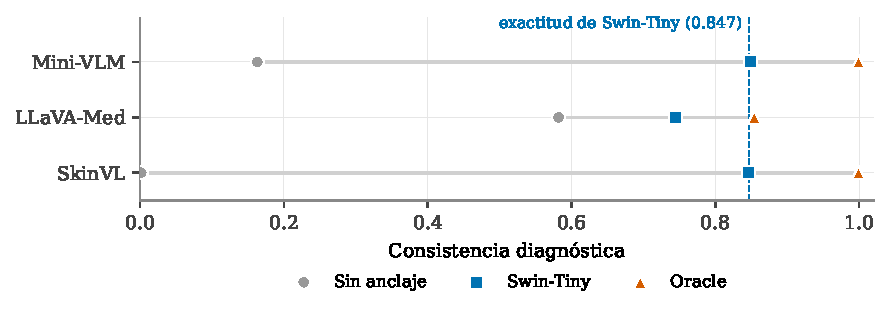
\includegraphics[width=\textwidth]{Figures/Capitulos/05-Resultados-Generacion/cascada-fuentes.pdf}
    \caption{Consistencia diagnóstica de cada generador según la fuente del diagnóstico. La línea discontinua es la
    exactitud de Swin-Tiny.}
    \label{fig:res_gen_cascada}
\end{figure}

\begin{table}[H]
    \centering
    \caption{Consistencia diagnóstica de la cascada según la fuente del diagnóstico, con las diferencias y su IC del
    95\,\% (bootstrap pareado).}
    \label{tab:res_gen_cascada}
    \small
    \setlength{\tabcolsep}{2pt}
    \begin{tabularx}{\textwidth}{@{}>{\raggedright\arraybackslash}X cccccc@{}}
        \toprule
        \textbf{Generador} & \textbf{\encabezado{Sin\\anclaje}} & \textbf{DermLIP} & \textbf{\encabezado{Swin-\\Tiny}}
            & \textbf{Oracle} & \textbf{\encabezado{Swin-Tiny $-$\\sin anclaje}} & \textbf{\encabezado{Oracle $-$\\Swin-Tiny}} \\
        \midrule
        Mini-VLM & 0.163 & 0.717 & 0.849 & 0.999 & $+0.686$ [$+0.658$, $+0.712$] & $+0.150$ [$+0.132$, $+0.168$] \\
        LLaVA-Med & 0.582 & 0.641 & 0.745 & 0.854 & $+0.162$ [$+0.130$, $+0.194$] & $+0.110$ [$+0.094$, $+0.126$] \\
        SkinVL & 0.001 & 0.716 & 0.846 & 0.999 & $+0.845$ [$+0.827$, $+0.863$] & $+0.153$ [$+0.135$, $+0.171$] \\
        \bottomrule
    \end{tabularx}
\end{table}

Que la consistencia coincida con la exactitud del clasificador se explica porque los generadores copian el diagnóstico
que reciben. Mini-VLM nombra el diagnóstico de Swin-Tiny en todos los reportes salvo dos. Cuando ese diagnóstico es
correcto, el reporte nombra la clase verdadera en 1\,272 de 1\,273 imágenes, y cuando es incorrecto, solo en 4 de
230. Por lo tanto, en la cascada la fidelidad diagnóstica del reporte es la exactitud del clasificador, y la distancia
al oracle mide sus errores y no los del generador.

LLaVA-Med es la excepción, porque no siempre transcribe el diagnóstico. Aun con el oracle, uno de cada siete
reportes no nombra la clase recibida. La mayoría describe la lesión y termina sin enunciar ningún diagnóstico, a pesar
de que la instrucción lo pide, y el resto son textos demasiado breves, entre ellos los que quedan vacíos cuando el
límite de tokens corta un bloque de razonamiento. Estas omisiones se concentran en \gls{nv}, \gls{bkl} y \gls{akiec}, y
son fallas del generador y no del clasificador (Sección~\ref{sec:res_gen_errores}).

La misma relación aparece cuando la fuente es DermLIP sin ajuste, el \gls{vlm} de la Sección~\ref{sec:res_vlm}, que
acierta en 0.716 de las imágenes de la prueba. Mini-VLM y SkinVL nombran el diagnóstico de DermLIP en todos los
reportes salvo uno y dos, respectivamente, y su consistencia coincide con esa exactitud. Por lo tanto, el generador
transcribe el diagnóstico de igual modo cuando proviene de un clasificador ajustado y cuando proviene de un modelo
sin ajuste, y la fidelidad del reporte es la de la fuente.

Lo que cambia con la fuente es cuántos errores se transcriben. Con Mini-VLM, la cascada con Swin-Tiny supera a la de
DermLIP en 0.132 [0.107, 0.158] de consistencia, y la diferencia es similar con los otros dos generadores. LLaVA-Med,
además, apenas mejora con DermLIP frente a no anclar, porque sigue omitiendo el diagnóstico recibido en uno de cada
siete reportes. Por lo tanto, de las dos fuentes que no conocen la etiqueta, el clasificador ajustado es la que lleva
más diagnósticos correctos al reporte.

\subsection{Consistencia por clase}
\label{sec:res_gen_clases}

Si el generador copia el diagnóstico, la cascada hereda también la sensibilidad de Swin-Tiny en cada clase. La
Figura~\ref{fig:res_gen_clases} lo confirma: con Mini-VLM y SkinVL, la consistencia de cada clase coincide con la
sensibilidad del clasificador en esa clase, de modo que los puntos quedan sobre la diagonal. LLaVA-Med queda por debajo
en casi todas las clases, y la mayor pérdida está en \gls{akiec}, donde nombra la clase en la mitad de los reportes en
que el clasificador la acierta.

\begin{figure}[H]
    \centering
    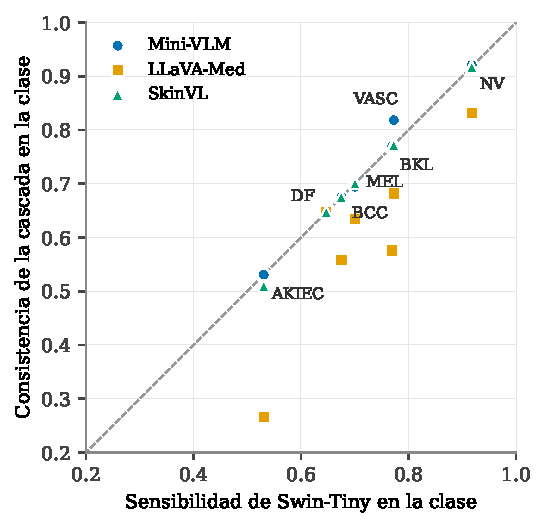
\includegraphics[width=0.62\textwidth]{Figures/Capitulos/05-Resultados-Generacion/cascada-por-clase.pdf}
    \caption{Sensibilidad de Swin-Tiny en cada clase frente a la consistencia de la cascada en esa clase.}
    \label{fig:res_gen_clases}
\end{figure}

La consecuencia clínica es que la cascada reproduce los puntos débiles del clasificador. Con la semilla que ancla el
pipeline, Swin-Tiny reconoce siete de cada diez melanomas, algo más que la media de sus tres semillas
(Sección~\ref{sec:res_melanoma}), y por ello tres
de cada diez reportes de un melanoma no lo nombran. Las clases con menor sensibilidad, como \gls{akiec},
reciben del mismo modo los reportes menos fieles, de modo que mejorar el reporte de una clase exige mejorar el
diagnóstico que lo ancla.

\subsection{Aporte de la imagen al reporte}
\label{sec:res_gen_ablaciones}

Si la fidelidad del reporte viene del clasificador, queda por saber qué hace el generador con la imagen. Para
responderlo, la cascada con el oracle se repitió en las dos variantes de la
Sección~\ref{sec:met_referencias}: con la imagen reemplazada por una gris neutra y con un diagnóstico equivocado, como
\gls{mel} por \gls{nv}. La Tabla~\ref{tab:res_gen_ablaciones} reúne los resultados, sobre 400 imágenes con Mini-VLM y
LLaVA-Med y sobre la prueba completa con SkinVL.

\begin{table}[H]
    \centering
    \caption{Cascada con el oracle con la imagen, sin ella y con un diagnóstico equivocado. La consistencia se
    mide respecto de la clase verdadera.}
    \label{tab:res_gen_ablaciones}
    \small
    \setlength{\tabcolsep}{3pt}
    \begin{tabularx}{\textwidth}{@{}>{\raggedright\arraybackslash}X cccccc@{}}
        \toprule
        & & \multicolumn{3}{c}{\textbf{Consistencia diagnóstica}} & \textbf{\encabezado{Reportes\\distintos}}
            & \textbf{\encabezado{Cobertura\\de entidades}} \\
        \cmidrule(lr){3-5}
        \textbf{Generador} & \textbf{Imágenes} & \textbf{\encabezado{Con\\imagen}} & \textbf{\encabezado{Sin\\imagen}}
            & \textbf{\encabezado{Diagnóstico\\equivocado}} & \textbf{\encabezado{Con / sin\\imagen}}
            & \textbf{\encabezado{Con / sin\\imagen}} \\
        \midrule
        Mini-VLM & 400 & 1.000 & 1.000 & 0.000 & 395 / 7 & 0.787 / 0.378 \\
        LLaVA-Med & 400 & 0.863 & 0.893 & 0.020 & 399 / 7 & 0.760 / 0.811 \\
        SkinVL & 1\,503 & 0.999 & 0.967 & 0.000 & 67 / 7 & 0.377 / 0.423 \\
        \bottomrule
    \end{tabularx}
\end{table}

La imagen no interviene en qué diagnóstico afirma el reporte. Sin ella, la consistencia no cambia con Mini-VLM, con
LLaVA-Med sube tres centésimas sin que la diferencia se distinga de cero, y con SkinVL baja apenas tres centésimas. Con un diagnóstico equivocado, en cambio, la consistencia cae a
cero en los tres generadores, porque el reporte afirma el diagnóstico recibido y no lo corrige a partir de la imagen:
Mini-VLM nombra la clase equivocada en todos los reportes y LLaVA-Med, en tres de cada cuatro. En consecuencia, un
error del clasificador llega al reporte sin ninguna corrección.

La imagen sí interviene en qué se describe. Sin ella, los tres generadores escriben un único texto por clase, siete
por generador, mientras que con ella casi cada reporte de Mini-VLM y de LLaVA-Med es distinto. Además, la cobertura de entidades
clínicas de Mini-VLM cae a la mitad sin la imagen, de modo que su descripción se apoya en ella. En LLaVA-Med, en cambio,
la cobertura no baja, porque sin la imagen el generador escribe una descripción genérica de la clase, con tantos
términos clínicos como la de una lesión concreta. Por lo tanto, el clasificador aporta el diagnóstico, y la imagen
aporta la variación de la descripción entre lesiones, aunque estas métricas no permiten saber si lo descrito está en la imagen
(Sección~\ref{sec:met_eval_generacion}).

\subsection{Fallas de los reportes}
\label{sec:res_gen_errores}

La consistencia indica si el reporte nombra la clase verdadera, pero no de qué manera falla cuando no lo hace. Para
saberlo, cada reporte se asignó a su falla principal con las reglas de la Sección~\ref{sec:met_eval_generacion}, que
cuentan aparte la expresión de reserva junto a la clase verdadera, como «consistent with nevus», porque el reporte se
compromete con el diagnóstico. La Figura~\ref{fig:res_gen_errores} muestra la distribución de las fallas de cada
generador sin anclaje, con Swin-Tiny y con el oracle.

\begin{figure}[H]
    \centering
    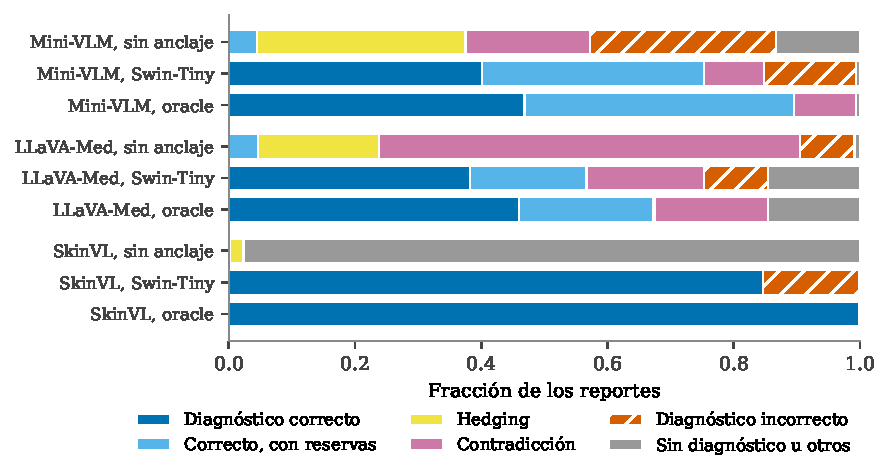
\includegraphics[width=\textwidth]{Figures/Capitulos/05-Resultados-Generacion/fallas-reportes.pdf}
    \caption{Falla principal de los reportes de cada generador según la fuente del diagnóstico.}
    \label{fig:res_gen_errores}
\end{figure}

Sin anclaje, cada generador tiene un patrón de fallas distinto. Dos de cada tres reportes de LLaVA-Med son contradicciones,
porque enumeran varias clases, y Mini-VLM reparte sus fallas entre el hedging y el diagnóstico incorrecto, que
juntos reúnen casi dos tercios de sus reportes. SkinVL, por su parte, no nombra ninguna clase en casi ningún reporte.
Estas distribuciones explican las consistencias de la Tabla~\ref{tab:res_gen_sin_anclaje}: la de LLaVA-Med proviene
de enumerar y no de afirmar el diagnóstico.

Con el anclaje, el hedging desaparece en los tres generadores, y el diagnóstico incorrecto queda reducido a los
errores del clasificador. Con el oracle, el diagnóstico incorrecto desaparece, y lo que queda son fallas del
generador. En Mini-VLM, uno de cada diez reportes nombra además otra clase, mientras que en LLaVA-Med casi uno de cada
cinco es una contradicción y uno de cada diez no nombra ninguna clase. SkinVL no tiene más fallas que las del
clasificador, porque escribe una oración breve con el diagnóstico recibido. La repetición, frecuente con la
decodificación voraz (Sección~\ref{sec:marco_rep_fallas}), afecta al 4\,\% de los reportes de Mini-VLM sin anclaje y a
menos del 1\,\% con anclaje.

\subsection{Recuperación de casos parecidos}
\label{sec:res_gen_rag}

La cascada depende de un clasificador entrenado, y la recuperación de la Sección~\ref{sec:met_recuperacion} es la
alternativa que entrega al generador los diagnósticos de los tres casos de entrenamiento más parecidos. La
Tabla~\ref{tab:res_gen_rag} la compara con la cascada en Mini-VLM, junto con dos líneas base sin generador que
escriben solo el diagnóstico: el voto del \gls{knn} y el de Swin-Tiny. Además de la consistencia, la tabla informa la
proporción de reportes que nombran la clase verdadera y ninguna otra.

\begin{table}[H]
    \centering
    \caption{Recuperación frente a la cascada en Mini-VLM.}
    \label{tab:res_gen_rag}
    \small
    \begin{tabularx}{\textwidth}{@{}>{\raggedright\arraybackslash}X >{\centering\arraybackslash}p{3.0cm}
        >{\centering\arraybackslash}p{3.0cm}@{}}
        \toprule
        \textbf{Condición} & \textbf{Consistencia diagnóstica} & \textbf{Solo la clase verdadera} \\
        \midrule
        Sin anclaje & 0.163 & 0.045 \\
        Recuperación sola & 0.669 & 0.500 \\
        Voto del \gls{knn}, sin generador & 0.781 & 0.781 \\
        Cascada con Swin-Tiny & 0.849 & 0.757 \\
        Swin-Tiny, sin generador & 0.847 & 0.847 \\
        Cascada con Swin-Tiny y recuperación & 0.862 & 0.792 \\
        \bottomrule
    \end{tabularx}
\end{table}

La recuperación sola mejora mucho la consistencia frente a no anclar, pero no reemplaza al clasificador. Queda casi
dos décimas por debajo de la cascada con Swin-Tiny, y también por debajo de escribir directamente el voto del
\gls{knn}. Es decir, el generador aprovecha peor la información de los vecinos que una regla de votación: cuando los
tres no coinciden, nombra varias clases o una distinta, y por eso solo la mitad de sus reportes nombra únicamente la
clase verdadera.

Sumar la recuperación a la cascada, por su parte, aporta poco. La consistencia sube 0.013 [0.007, 0.019], pero la
ganancia viene de que el reporte agrega la clase de los vecinos cuando difiere de la del clasificador, de modo que
nombra más candidatos: escribir solo el diagnóstico de Swin-Tiny da reportes más exclusivos. Tampoco un vecino
equivocado degrada el reporte. En las 171 imágenes en que Swin-Tiny acierta y el voto del \gls{knn} no, la cascada con
recuperación nombra la clase verdadera en todos los reportes, igual que sin ella, y en las 72 en que ocurre lo
contrario, recupera la clase verdadera en una de cada seis. El generador, por lo tanto, sigue al diagnóstico del
clasificador también cuando recibe otra evidencia.

En síntesis, la cascada lleva al reporte la exactitud del clasificador junto con sus errores, y ni la imagen ni los
casos recuperados corrigen esos errores. La sección siguiente evalúa si la concordancia entre el clasificador y el
\gls{knn} permite reconocer los casos en que el diagnóstico es menos confiable.
